\section{Parallele Modelle}

\subsection{Circuit}
%----------------------------------------------------------------------%SLIDE -
\begin{frame}
    \frametitle{Circuit}
    \begin{itemize}
        \item ein gerichteter, azyklischer Graph (DAG)
        \item Eingabe, Ausgabe
        \item Operationen
        \item Boolean Circuit
    \end{itemize}
\end{frame}
%----------------------------------------------------------------------%SLIDE -

%----------------------------------------------------------------------%SLIDE -
\begin{frame}[b]
    \frametitle{Boolean Circuit}
    \framesubtitle{Addition von acht Zahlen}
    \begin{columns}[b]
        \column{0.5\textwidth}
        \begin{figure}
            \centering
            % sequential circuit computing the sum of eight numbers
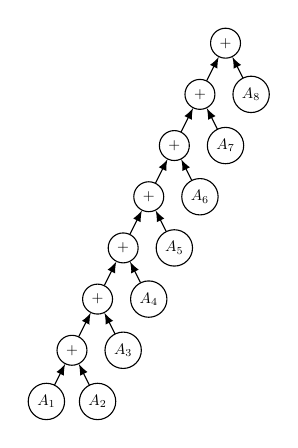
\begin{tikzpicture}
    [
        vertex/.style={circle, draw, scale=0.55, minimum size=3ex,},
        edge/.style={-latex,},
        scale=0.65,
    ]

    % sequential dag
    \node (b1) at (-3,0)    [vertex] {$A_1$};
    \node (b2) at (-2,0)    [vertex] {$A_2$};

    \node (q1) at (-2.5,1)  [vertex] {$+$};
    \node (b3) at (-1.5,1)  [vertex] {$A_3$};

    \node (q2) at (-2,2)    [vertex] {$+$};
    \node (b4) at (-1,2)    [vertex] {$A_4$};

    \node (q3) at (-1.5,3)  [vertex] {$+$};
    \node (b5) at (-0.5,3)  [vertex] {$A_5$};

    \node (q4) at (-1,4)    [vertex] {$+$};
    \node (b6) at (0,4)     [vertex] {$A_6$};

    \node (q5) at (-0.5,5)  [vertex] {$+$};
    \node (b7) at (0.5,5)   [vertex] {$A_7$};

    \node (q6) at (0,6)     [vertex] {$+$};
    \node (b8) at (1,6)     [vertex] {$A_8$};

    \node (q7) at (0.5,7)   [vertex] {$+$};

    \draw [edge] (b1) -- (q1);
    \draw [edge] (b2) -- (q1);
    \draw [edge] (b3) -- (q2);
    \draw [edge] (b4) -- (q3);
    \draw [edge] (b5) -- (q4);
    \draw [edge] (b6) -- (q5);
    \draw [edge] (b7) -- (q6);
    \draw [edge] (b8) -- (q7);
    \draw [edge] (q1) -- (q2);
    \draw [edge] (q2) -- (q3);
    \draw [edge] (q3) -- (q4);
    \draw [edge] (q4) -- (q5);
    \draw [edge] (q5) -- (q6);
    \draw [edge] (q6) -- (q7);

\end{tikzpicture}         

            \caption{eine Möglichkeit}
        \end{figure}
        \pause
        \column{0.5\textwidth}
        \begin{figure}
            \centering
            % parallel circuit computing the sum of eight numbers
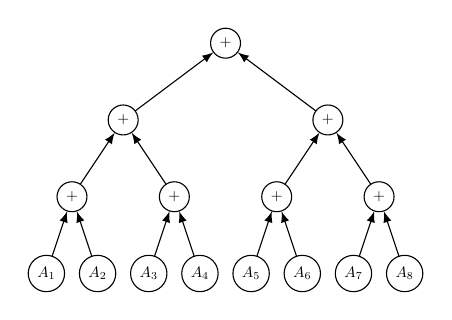
\begin{tikzpicture}
    [
        vertex/.style={circle, draw, scale=0.55, minimum size=3ex,},
        edge/.style={-latex,},
        scale=0.65,
    ]

    % parallel dag
    \node (a1) at (0,0)     [vertex] {$A_1$};
    \node (a2) at (1,0)     [vertex] {$A_2$};
    \node (a3) at (2,0)     [vertex] {$A_3$};
    \node (a4) at (3,0)     [vertex] {$A_4$};
    \node (a5) at (4,0)     [vertex] {$A_5$};
    \node (a6) at (5,0)     [vertex] {$A_6$};
    \node (a7) at (6,0)     [vertex] {$A_7$};
    \node (a8) at (7,0)     [vertex] {$A_8$};
    \node (p1) at (0.5,1.5) [vertex] {$+$};
    \node (p2) at (2.5,1.5) [vertex] {$+$};
    \node (p3) at (4.5,1.5) [vertex] {$+$};
    \node (p4) at (6.5,1.5) [vertex] {$+$};
    \node (p5) at (1.5,3)   [vertex] {$+$};
    \node (p6) at (5.5,3)   [vertex] {$+$};
    \node (p7) at (3.5,4.5) [vertex] {$+$};
    \draw [edge] (a1) -- (p1);
    \draw [edge] (a2) -- (p1);
    \draw [edge] (a3) -- (p2);
    \draw [edge] (a4) -- (p2);
    \draw [edge] (a5) -- (p3);
    \draw [edge] (a6) -- (p3);
    \draw [edge] (a7) -- (p4);
    \draw [edge] (a8) -- (p4);
    \draw [edge] (p1) -- (p5);
    \draw [edge] (p2) -- (p5);
    \draw [edge] (p3) -- (p6);
    \draw [edge] (p4) -- (p6);
    \draw [edge] (p5) -- (p7);
    \draw [edge] (p6) -- (p7);

\end{tikzpicture}         

            \caption{eine andere}
        \end{figure}
    \end{columns}
\end{frame}
%----------------------------------------------------------------------%SLIDE -
